% Rebuilt with original Frontiers template files and user-locked final PNG figures on 2026-07-07.
% Official Frontiers LaTeX template version.
        % Target journal: Frontiers in Signal Processing, Biomedical Signal Processing specialty.
        \documentclass[utf8]{FrontiersinHarvard}

        \usepackage{url,hyperref,lineno,microtype,subcaption}
        \hypersetup{hidelinks}
        \usepackage[singlespacing]{setspace}
        \usepackage{graphicx}
        \usepackage{booktabs}
        \usepackage{longtable}
        \usepackage{array}
        \usepackage{amsmath,amssymb}

        \linenumbers

        \def\keyFont{\fontsize{8}{11}\helveticabold }
        \def\firstAuthorLast{Gui {et~al.}}
        \def\Authors{Xiaoqian Gui\,$^{1,\dagger}$, Kaisi Zhu\,$^{2,\dagger}$, Ziyi Jiang\,$^{3,\dagger}$ and Feifan Lu\,$^{4,*}$}
        \def\Address{$^{1}$Changhai Center for Simulation, Learning and Innovation, Changhai Hospital, Naval Medical University, Shanghai, China \\
$^{2}$Department of Anesthesiology, Changhai Hospital, Naval Medical University, Shanghai, China \\
$^{3}$Department of General Internal Medicine, The 929th Hospital, Affiliated with Changhai Hospital, Naval Medical University, China \\
$^{4}$Department of Obstetrics and Gynecology, Changhai Hospital, Naval Medical University, Shanghai, China}
        \def\corrAuthor{Feifan Lu}
        \def\corrEmail{luff94@163.com}

        \begin{document}
        \onecolumn
        \firstpage{1}

        \title[Self-supervised CTG signal representation]{Self-supervised biomedical signal representation learning from intrapartum cardiotocography for neonatal risk enrichment}

        \author[\firstAuthorLast ]{\Authors}
        \address{}
        \correspondance{}

        \extraAuth{$^\dagger$ These authors have contributed equally to this work.}

        \maketitle

        \begin{abstract}
        \section{}
        Intrapartum cardiotocography (CTG) records long paired fetal heart rate (FHR) and uterine contraction (UC) signals, but many decision-support approaches still compress these physiological trajectories into static summaries. We evaluated whether self-supervised learning (SSL) for biomedical signal representation can support interpretable neonatal risk enrichment using open CTG data. CTU-UHB/CTU-CHB was used as the primary raw-signal cohort and CTGDL-FHRMA for external representation/domain-shift analysis. The primary endpoint was umbilical artery pH $<$7.15 or 5-minute Apgar score $<$7. CTU-UHB records were split at the record level into 386 training and 166 held-out test records. A compact PatchTST-style transformer encoder was trained only on training-record FHR and UC windows using patch tokenization, masked reconstruction and NT-Xent contrastive consistency, and record-level embeddings were combined with classical signal features and dynamic phenotypes. In the held-out test set, signal-only features achieved an area under the precision-recall curve (AUPRC) of 0.3366 (95\% CI 0.2173--0.4941). In the seeded locked replay, adding self-supervised embeddings yielded AUPRC 0.3765 (95\% CI 0.2399--0.5243), and the signal-plus-embedding-plus-phenotype model achieved an area under the receiver-operating-characteristic curve (AUROC) of 0.6168 (95\% CI 0.5111--0.7191) and AUPRC 0.4016 (95\% CI 0.2605--0.5471). Both SSL-containing AUPRC-difference intervals versus signal-only features crossed zero, so SSL is framed as an interpretable representation, phenotype-enrichment and recalibration layer rather than as a stable discrimination-improvement result. Development-only model selection gave a conservative held-out AUPRC of 0.3872. Cross-fitted Platt recalibration improved Brier score from 0.2652 to 0.1566, and CTGDL-FHRMA showed substantial representation domain shift (domain AUROC 0.9088). These findings support SSL-based CTG representation learning as a reproducible biomedical signal-processing workflow for hypothesis-generating risk enrichment and phenotype discovery, but they do not establish external clinical validity or clinical deployability.

        \tiny
        \keyFont{ \section{Keywords:} cardiotocography, biomedical signal processing, self-supervised learning, time-series representation learning, fetal heart rate, uterine contraction, neonatal risk, calibration}
        \end{abstract}

        \section{Introduction}

Intrapartum cardiotocography (CTG) monitoring is widely used to assess fetal status during labour, but its clinical value and interpretation remain contested because visual assessment has limited positive predictive value and substantial observer variability \citep{alfirevic2017,figo2015,nichd2008,francis2024}. The clinical decision problem is not merely whether an algorithm can assign a label after delivery. During labour, CTG interpretation may influence closer surveillance, escalation, fetal blood sampling where available, operative delivery or reassurance. A useful informatics model should therefore help enrich risk and explain signal patterns without replacing obstetric judgement. The raw CTG signal is inherently dynamic: fetal heart rate (FHR) and uterine contraction (UC) traces record how the fetus responds to contractions and changing intrapartum stress over time. In practice, however, this temporal information is often compressed into static summary features, categorical rule systems or visual interpretation. Such compression can support standardisation, but it may also discard trajectory structure that is relevant for decision-oriented risk enrichment and phenotype discovery \citep{mendis2023}.

Self-supervised learning (SSL) time-series models provide a possible route from raw physiological trajectories to reusable representations, consistent with the broader foundation-model direction in medicine and with recent transformer-based time-series representation learning \citep{moor2023,zerveas2021,nie2023,yue2022,goswami2024moment}. Recent open-source time-series methods converge on design principles that are well matched to CTG. Patch-level tokenisation can reduce long FHR/UC windows to tractable temporal tokens while preserving local morphology. Random, block, mixed and channel-level masking strategies can expose the encoder to signal loss, temporal corruption and channel-specific degradation, all of which resemble practical CTG artefact and monitoring interruptions. Masked reconstruction then forces the model to recover missing trajectory structure, whereas contrastive objectives encourage embeddings from augmented views of the same underlying record to remain close \citep{nie2023,yue2022,zhang2022tfc}. For obstetric CTG, however, the relevant question is not simply whether a deep model can predict an adverse neonatal label. A credible workflow also has to show that learned representations add information beyond classical signal summaries, that dynamic phenotypes remain clinically interpretable, that absolute risks can be recalibrated, and that external public data are used within their legitimate outcome-label boundaries \citep{tripodai2024,vanCalster2019,vickers2006}. These requirements are especially important for open-data studies, where external datasets may support representation transport or domain-shift assessment without supporting external clinical outcome validation.

Large supervised CTG interpretation studies define a complementary benchmark. In a nationwide multicentre study, Park et al. used 22,522 deliveries from 14 hospitals and 519,800 person-minutes of CTG to train an SE-ResNet50-based normal-versus-abnormal CTG classifier, reporting internal AUROC/PRC of 0.880/0.625 and three external AUROCs of 0.862, 0.895 and 0.862 \citep{park2025nationwide}. Concurrent preprint work has also explored larger CTG foundation-model and multi-view SSL pretraining systems \citep{fridman2026ctgfoundation,prismctg2026}. These studies use different training scales, downstream tasks and validation settings, so they provide context rather than a direct head-to-head benchmark. The present work addresses a narrower open-data problem: whether raw FHR/UC trajectories can yield reusable self-supervised representations, clinically inspectable phenotypes, calibrated neonatal-risk enrichment and honest domain-shift assessment when large proprietary annotated datasets are unavailable. Rather than presenting another claim of deployable fetal-stress prediction, we developed an open-data CTG decision-modelling workflow using CTU-UHB/CTU-CHB as the primary raw-signal cohort and CTGDL-FHRMA as an external representation-assessment resource \citep{goldberger2000,chudacek2014,ctuuhb,ctgdl}. We trained a compact PatchTST-style masked transformer encoder on FHR and UC windows, derived both signal-based and SSL-based phenotypes, and evaluated neonatal risk enrichment using a fixed record-level split. The analysis combined bootstrap confidence intervals, permutation-based explanation, missingness sensitivity, cross-fitted recalibration, decision curve analysis and external domain-shift assessment. Given the small cohort and low event-to-predictor ratio, this design was intended to test whether self-supervised CTG representations can support a bounded, reproducible and clinically legible phenotyping-and-calibration workflow for later validation, rather than to claim an autonomous clinical risk calculator.

\section{Results}

\subsection{Open CTG data defined a leakage-aware phenotyping workflow}

To establish the analysis frame, we used CTU-UHB/CTU-CHB as the primary raw-signal cohort and retained CTGDL-FHRMA for external representation assessment. CTU-UHB records were split at the record level into 386 training records and 166 held-out test records, before any downstream window-level modelling. This design reduced leakage between overlapping windows from the same CTG record and approximated a future-record evaluation setting, which is more relevant to decision modelling than random window-level splitting. The resulting workflow linked raw FHR/UC signals to dynamic representations, phenotypes, risk prediction, recalibration and external domain-shift analysis (Figure 1).
% ===== FIGURE 1 INSERTION POINT =====
% Production note: insert Figure 1 near the preceding paragraph.


\subsection{Self-supervised representations provided a bounded enrichment and interpretation layer}

To test whether learned trajectory representations added value beyond classical CTG summaries, we compared signal-only, SSL-augmented and phenotype-augmented models in the held-out CTU-UHB test set. The neonatal-risk endpoint occurred in 79 of 386 training records (20.47\%) and 34 of 166 held-out test records (20.48\%). Signal-only features achieved an AUPRC of 0.3366 (95\% CI 0.2173--0.4941), corresponding to 1.64-fold enrichment over the held-out event prevalence. Fold-enrichment denotes AUPRC divided by event prevalence, the expected AUPRC of a random classifier. As an ablation, SSL embeddings alone achieved AUPRC 0.2125 and AUROC 0.4947, indicating that the learned representation was not sufficient as a stand-alone predictor in this small labelled cohort. In the seeded locked replay, combining transformer SSL embeddings with signal features yielded AUPRC 0.3765 (95\% CI 0.2399--0.5243), corresponding to 1.84-fold enrichment, with a bootstrap AUPRC difference of 0.0310 (95\% CI -0.0527--0.1077) versus signal-only features. The primary manuscript model, which combined signal features, SSL embeddings and signal phenotypes, achieved an AUROC of 0.6168 (95\% CI 0.5111--0.7191) and an AUPRC of 0.4016 (95\% CI 0.2605--0.5471), corresponding to 1.96-fold enrichment over prevalence. Its AUPRC difference versus signal-only features was 0.0548 (95\% CI -0.0354--0.1519). Because both SSL-containing AUPRC-difference intervals crossed zero, the phenotype-augmented model is retained for interpretation, phenotype analysis and recalibration, not because it establishes a statistically resolved AUPRC improvement. Because the compact transformer ranking used held-out AUPRC for method exploration, we performed an additional development-only model-selection sensitivity analysis within the original training records. In that analysis, a 75\%/25\% stratified split of the training records selected the smaller p80-d48-l2 mixed-masking signal-plus-SSL-plus-signal-phenotype configuration; when fitted on all original training records and evaluated once in the held-out test set, this development-selected configuration achieved an AUROC of 0.6348, AUPRC of 0.3872 and Brier score of 0.2542. We therefore interpret the held-out-ranked transformer comparison as exploratory and regard the development-selected result as a conservative enrichment estimate (Supplementary Table S9). This pattern is important for clinical decision relevance because a low-prevalence neonatal risk task is often used for enrichment or triage rather than definitive diagnosis. AUPRC directly reflects how well high-scoring records concentrate true adverse outcomes among records selected for attention, whereas AUROC can remain insensitive to clinically relevant changes in the high-risk tail. In this replay-locked analysis, AUPRC, AUROC and Brier-score differences crossed zero, indicating that SSL should be interpreted as an interpretable representation and enrichment layer rather than as broad improvement in discrimination or raw calibration (Figure 2A--D; Supplementary Figure S1A,B).
% ===== FIGURE 2 INSERTION POINT =====
% Production note: insert Figure 2 near the preceding paragraph.


The model-validation evidence is summarized in Figure 2, including held-out precision-recall and receiver-operating-characteristic curves, bootstrap model comparisons, missingness sensitivity and feature-importance results.

Permutation analysis supported a mixed clinical and representation-based signal. In the signal-plus-SSL model, the positive AUPRC importance sum was 0.4874 for clinical signal features and 2.6003 for SSL embedding dimensions. Mean positive AUPRC importance per feature was similar across the two families (0.0406 and 0.0406, respectively), suggesting that the representation contribution was distributed across multiple embedding dimensions rather than driven by a single latent variable (Figure 2F; Supplementary Figure S1D).

Because FHR missingness contributed to prediction, models were rerun after excluding FHR and UC missingness fractions. Without missingness features, signal plus SSL achieved an AUPRC of 0.3951 (95\% CI 0.2507--0.5470), and the final model achieved an AUPRC of 0.3982 (95\% CI 0.2537--0.5486). The no-missingness AUPRC difference for the final model versus signal-only features was 0.0132 (95\% CI -0.0691--0.0894). These results show that the representation layer remained usable after removing explicit missingness fractions, but they do not establish a statistically secure missingness-independent gain (Figure 2E). To address the high-dimensionality concern, we repeated the final model using principal components of the SSL embeddings fitted within the training records. A 10-component SSL PCA representation explained 95.67\% of training embedding variance and achieved an AUPRC of 0.4241 with 23 predictors before one-hot expansion; a 20-component representation explained 99.53\% of variance and achieved an AUPRC of 0.4256 with 33 predictors. These dimensionality checks support the feasibility of lower-dimensional SSL summaries, but they remain exploratory and should not be read as a separate improvement claim. All event-to-predictor ratios remained low, so absolute performance estimates should be read as optimistic and hypothesis-generating (Supplementary Table S9).

The endpoint-threshold sensitivity analyses are summarized in Supplementary Figure S3 and supported the same enrichment direction but also illustrated the limits imposed by sparse severe events. For the pH-only endpoint pH $<$7.10, the held-out event prevalence was 11.45\% (19 events), and the final feature set achieved an AUPRC of 0.4870, or 4.25-fold enrichment over prevalence. For pH $<$7.05, the held-out event prevalence was 9.04\% (15 events), and the final feature set achieved an AUPRC of 0.5260, or 5.82-fold enrichment. These analyses were treated as sensitivity checks rather than definitive secondary endpoints because the severe-acidosis event counts were small (Supplementary Figure S3; Supplementary Table S9).

\subsection{Signal phenotypes anchored the latent model in CTG physiology}

To make the modelling output clinically legible, we derived signal-based phenotypes and selected representative prototype records. The four signal-derived phenotypes showed interpretable differences in neonatal risk and CTG signal profiles. Signal phenotype 2 had the highest neonatal risk rate (0.3439), lower mean cord pH (7.1877), higher FHR standard deviation (22.2159) and higher deceleration-proxy burden (3530.4777). This profile is consistent with a subgroup in which fetal heart rate responses to uterine activity are more unstable and deceleration-prone, although the retrospective data do not prove a causal fetal-distress mechanism. Signal phenotype 4 had the lowest neonatal risk rate (0.1048). Prototype records illustrated the paired FHR and UC patterns underlying each phenotype (Figure 3).
% ===== FIGURE 3 INSERTION POINT =====
% Production note: insert Figure 3 near the preceding paragraph.
 These results positioned signal phenotypes as the main clinical interpretation layer for the SSL-enhanced model: the latent encoder contributed risk information, while phenotype prototypes translated part of that information into recognizable CTG trajectory patterns.

\subsection{Platt recalibration improved absolute risk estimates and threshold behavior}

The calibration and decision-curve analyses are summarized in Figure 4. Because risk enrichment alone does not make a clinically usable probability, we next evaluated calibration and threshold behaviour. Raw deep-model scores should not be interpreted as absolute neonatal risk, particularly when the development cohort, outcome definition and signal quality differ from future clinical settings. Raw predictions from the final signal-plus-SSL-plus-signal-phenotype model were poorly calibrated. The raw Brier score was 0.2652 (95\% CI 0.2260--0.3020), raw calibration intercept was -1.3588 (95\% CI -1.8087 to -0.9874), raw calibration slope was 0.3448 (95\% CI 0.0861--0.6295), and raw expected calibration error was 0.2568 (95\% CI 0.2083--0.3374). Cross-fitted Platt recalibration improved the Brier score to 0.1566 (95\% CI 0.1254--0.1916), calibration intercept to 0.0770 (95\% CI -1.0397 to 1.1445), and calibration slope to 1.1649 (95\% CI 0.2914--2.1251). The held-out expected calibration error decreased to 0.0322; because expected calibration error is bin-dependent and bootstrap samples altered bin composition, the bootstrap mean was 0.0648 (95\% CI 0.0284--0.1098). Bootstrap differences for Platt minus raw predictions were -0.1085 for Brier score (95\% CI -0.1516 to -0.0643) and -0.2050 for expected calibration error (95\% CI -0.2588 to -0.1294). In the 0.10--0.30 threshold range, mean net benefit increased from 0.0261 for raw predictions to 0.0442 after Platt recalibration. Isotonic recalibration improved some calibration metrics but reduced AUPRC, so it was treated as exploratory (Figure 4). These findings make recalibration a necessary decision-modelling step rather than a cosmetic post-processing analysis.
% ===== FIGURE 4 INSERTION POINT =====
% Production note: insert Figure 4 near the preceding paragraph.


\subsection{CTGDL-FHRMA showed representation transport with substantial domain shift}

Finally, we examined whether the trained representation could be projected onto an external open CTG resource. External CTGDL-FHRMA analysis included 135 records and was compared with 552 CTU-UHB records in the transformer embedding space. The first two principal components explained 0.5092 of embedding variance. A CTU-versus-CTGDL domain classifier achieved an AUROC of 0.9088, indicating that CTU-UHB and CTGDL-FHRMA embeddings were almost fully separable and that the learned representation did not transport cleanly across these datasets. CTGDL-FHRMA records were assigned across CTU-derived SSL phenotypes, with most assigned to phenotypes 1 and 3. Within CTU-UHB, the same SSL phenotype layer showed a rising neonatal-risk gradient (Supplementary Figure S2D), supporting phenotype ordering as source-cohort evidence while not replacing external outcome validation. We treated the CTGDL-FHRMA result as a prespecified boundary rather than a failed external validation exercise: because CTGDL-FHRMA did not provide the same neonatal outcome structure used in CTU-UHB, forcing an external outcome comparison would risk a misleading estimate of clinical generalisability. These analyses therefore support external representation projection with substantial domain-shift detection, not external clinical outcome validation or clean cross-dataset transportability (Supplementary Figure S2). Transformer model-selection and SSL phenotype sensitivity panels are provided as supplementary evidence for the final figure package (Supplementary Figure S1).

\section{Discussion}

This open-data CTG study demonstrates a bounded use case for self-supervised intrapartum trajectory modelling in biomedical signal processing. The main contribution is not a stand-alone clinical predictor, but a reproducible workflow that links masked time-series representations, clinically interpretable signal phenotypes, bootstrap validation, recalibration and external domain-shift assessment. This positioning is aligned with recent reviews emphasizing that automated CTG models require stronger generalisability, standardised outcome definitions and clearer translation pathways before clinical deployment \citep{mendis2023,francis2024}. In a decision-support context, the value of such a workflow lies in risk enrichment, signal explanation and calibration discipline rather than in replacing real-time obstetric judgement.

The most consistent signal was risk enrichment in AUPRC space under class imbalance, which matches the enrichment use case \citep{davis2006}; however, the increment was directionally consistent rather than statistically secure. In the locked replay, both SSL-containing AUPRC-difference intervals crossed zero, and the no-missingness final-model difference was 0.0132 (95\% CI -0.0691 to 0.0894). Because the transformer configuration was ranked on held-out AUPRC, the development-only selection (AUPRC 0.3872, AUROC 0.6348) remains an important conservative check. These results, together with an event-to-predictor ratio near one for the full SSL model, indicate that the findings should be read as hypothesis-generating representation and phenotype-enrichment evidence rather than as evidence of stable discrimination.

Compared with the nationwide supervised interpretation model reported by Park et al. \citep{park2025nationwide}, our dataset and validation scale are modest, and this manuscript should not be read as competing with multicentre external validation of expert-labelled abnormal CTG interpretation. Its contribution is complementary: a reproducible open-data method layer for self-supervised trajectory representation, phenotype prototypes, calibration-aware risk enrichment, decision-curve analysis and explicit representation-domain assessment.

The AI contribution should therefore be interpreted as a transparent representation-learning design rather than as a large-scale foundation model. PatchTST was chosen because patch tokenisation makes 10-minute two-channel CTG windows tractable while preserving local FHR and UC morphology, whereas sequence models over individual time points would be longer and less efficient for this open-data setting. Channel masking matched the final model's strongest sweep configuration and is clinically plausible because FHR or UC channels may degrade differently during monitoring; mixed and block masking were retained as sensitivity configurations. Masked reconstruction encouraged recovery of missing trajectory information, and the NT-Xent objective encouraged two augmented views of the same physiological record to occupy a consistent representation space. Phenotype clustering then converted part of the latent signal into inspectable prototypes and summaries. The contribution is therefore the integration of contemporary time-series SSL ingredients with dynamic phenotype discovery, leakage-aware validation, calibration, decision-curve analysis, missingness sensitivity and external representation-domain assessment.

\subsection{Clinical decision-support implications}

The intended clinical informatics role is risk enrichment and information organization, not autonomous diagnosis. A calibrated trajectory-representation workflow could, in principle, help investigators or future decision-support systems summarize long CTG records into inspectable phenotypes, identify records that warrant closer review, and communicate uncertainty on a probability scale after local recalibration. In the current study, these implications remain methodological because the model has not undergone institutionally external outcome validation or prospective workflow evaluation, and the absolute performance estimates are constrained by a low event-to-predictor ratio.

The phenotype analysis provides the main bridge between latent representations and clinical interpretation. Signal phenotype 2 combined higher neonatal risk (0.3439), lower mean cord pH (7.1877), greater FHR variability (FHR standard deviation 22.2159) and higher deceleration-proxy burden (3530.4777). This pattern is consistent with an intrapartum subgroup in which fetal cardiovascular responses to uterine activity are more unstable and deceleration-prone, but it should not be read as proof of a single pathophysiological mechanism. The value for decision informatics is that a clinician or investigator can inspect a prototype curve, signal summaries and model risk enrichment together, instead of receiving an opaque latent embedding alone. The workflow therefore separates representation learning from interpretation while allowing both layers to contribute to risk enrichment.

Recalibration materially changed the interpretation of the prediction scores. Cross-fitted Platt scaling improved Brier score and expected calibration error without altering the underlying ranking metrics. This distinction is central for clinical decision relevance. A high uncalibrated deep-model score may be useful for ranking records for attention, but it should not be communicated as an absolute probability of neonatal compromise. Platt recalibration provided a simple way to map the enrichment score onto a more interpretable probability scale under the fixed validation design. In the current sample, isotonic calibration was less attractive because it improved selected calibration summaries while reducing AUPRC.

Several limitations define the scope of these findings. The analysis was retrospective and public-data based, with only 552 CTU-UHB records and 79 training events; this is small for a transformer-derived, 64-dimensional embedding model and limits generalisation. CTGDL-FHRMA was used for representation projection and domain-shift assessment, not for external neonatal outcome validation, because outcome definitions, label availability and cohort structure were not sufficiently aligned. The domain-classifier AUROC of 0.9088 indicates that CTU-UHB and CTGDL-FHRMA embeddings were almost fully separable, so cross-dataset generalisation should not be assumed. The compact transformer sweep was exploratory and used held-out AUPRC for configuration ranking. For revision reproducibility, all performance estimates reported here come from the fixed-seed locked replay; the unseeded originally submitted values (signal+SSL AUPRC 0.4432 and final AUPRC 0.4324) were not retained because the exact run could not be reproduced. In the seeded locked replay, SSL-containing AUPRC differences versus signal-only features crossed zero, so SSL should not be interpreted as a stable discrimination-improvement component. PCA sensitivity analyses showed that lower-dimensional SSL summaries were feasible, but the event-to-predictor ratio remained low. Severe pH-threshold sensitivity analyses were directionally consistent but involved only 15--19 held-out events, and all sensitivity analyses were descriptive. Missingness remained influential, and after removing missingness features the SSL-containing differences remained statistically unresolved. The model and phenotype definitions therefore require institutionally external and prospective validation before clinical use.

In summary, open CTG data can support self-supervised dynamic phenotyping when the evidence chain includes leakage-aware splitting, baseline comparison, interpretability, calibration and domain-shift analysis. The present results justify further external validation of CTG trajectory phenotypes, but they should not be interpreted as sufficient evidence for clinical deployment.

\section{Methods}

\subsection{Study design and data sources}

This was a retrospective open-data modelling study of intrapartum cardiotocography. CTU-UHB/CTU-CHB was used as the primary raw-signal cohort because it provides FHR, UC, and clinical metadata for intrapartum records \citep{goldberger2000,chudacek2014,ctuuhb}. CTGDL-FHRMA was used for external representation and domain-shift analysis \citep{ctgdl}. UCI Cardiotocography was retained as a feature-level reference resource but was not used as raw-signal outcome validation \citep{uci}. Dataset URLs, access notes, and roles are summarized in Supplementary Table S1. Supplementary Table S2 reports held-out performance estimates; Supplementary Table S3 reports bootstrap model differences; Supplementary Table S4 provides phenotype summaries; Supplementary Table S5 provides prediction explainability outputs; Supplementary Table S6 reports missingness sensitivity; Supplementary Table S7 reports recalibration and decision-curve outputs; Supplementary Table S8 reports external representation analysis; Supplementary Table S9 reports reviewer-requested sensitivity analyses; Supplementary Table S10 provides the TRIPOD-AI reporting checklist; and Supplementary Table S11 provides the transformer hyperparameters.

\subsection{Outcome definition}

The primary endpoint was a binary composite neonatal-risk outcome defined at the CTU-UHB record level. A record was coded as positive if available metadata indicated umbilical artery pH $<$7.15 or 5-minute Apgar score $<$7. The pH threshold was chosen to define a broader at-risk acidemia group with sufficient event count for enrichment modelling in this open dataset and is consistent with prior CTU-UHB-oriented CTG modelling work \citep{chudacek2014,deepctg2023}. It was not intended to replace stricter definitions of severe metabolic acidosis; therefore, pH-only thresholds of $<$7.10 and $<$7.05 were evaluated as sensitivity analyses. The composite endpoint is clinically pragmatic but heterogeneous: umbilical artery pH captures acid-base status, whereas Apgar score can reflect non-hypoxic and transitional factors. Records not meeting either criterion were coded as non-events. Neonatal intensive care unit duration and other metadata fields were retained for cohort description where available but were not used in the primary composite endpoint. This definition yielded 113 positive records among 552 CTU-UHB records (20.47\%), including 79 of 386 training records (20.47\%) and 34 of 166 held-out test records (20.48\%).

\subsection{Record split and signal windowing}

Records were split at the record level into training and held-out test sets, following the principle that prediction-model validation must preserve independence between development and evaluation samples \citep{tripod2015,steyerberg2019,tripodai2024}. This split was applied before self-supervised pretraining, phenotype derivation, supervised model fitting, recalibration and held-out validation to prevent leakage between overlapping windows from the same CTG record. FHR and UC signals were converted into fixed-length windows using a target sampling rate of 4 Hz and 10-minute windows. The CTU-UHB corpus contained 7,602 windows, including 5,301 training-record windows and 2,301 held-out test-record windows. Transformer SSL pretraining used only training-record windows and did not use outcome labels. After the encoder was selected and fitted, clean unmasked windows from both splits were encoded for downstream record-level aggregation, with all supervised fitting restricted to the training records and all reported validation metrics computed in the held-out test records.

\subsection{AI model design rationale}

The deep-learning component was selected after reviewing open-source self-supervised time-series methods that could plausibly be reproduced in a public CTG study. PatchTST motivated the use of patch tokens and transformer encoding for long physiological sequences \citep{nie2023}. MOMENT and related time-series foundation-model work motivated masked patch reconstruction as a scalable pretext task \citep{goswami2024moment}. TS2Vec and TF-C motivated contrastive consistency as a complementary representation objective for downstream transfer \citep{yue2022,zhang2022tfc}. The design was adapted to the clinical signal problem rather than imported as a generic architecture: patching reduced long-window complexity, masking strategies approximated signal artefact and channel loss, reconstruction encouraged recovery of trajectory morphology, and contrastive consistency stabilized record-level embeddings across augmented views. We implemented these ingredients locally rather than importing external pretrained CTG weights, because the purpose of this manuscript was to evaluate a transparent, reproducible open-data phenotyping workflow under a fixed CTU-UHB split. The compact transformer sweep should be interpreted as an exploratory method-selection layer. To examine possible held-out selection bias, we added a development-only sensitivity analysis in which candidate configurations were ranked using only an internal split of the original training records, and the selected configuration was then evaluated once in the original held-out test set.

\subsection{Self-supervised time-series representation learning}

A PatchTST-style masked time-series transformer was trained on FHR and UC windows \citep{nie2023}. Each two-channel 10-minute window contained 2,400 time points per channel. The selected manuscript-candidate configuration used non-overlapping patches of length 80, with stride equal to patch length, yielding 30 temporal patches per channel and 60 channel-time tokens per window. Each patch was projected to a 64-dimensional latent token, combined with learnable positional and channel embeddings, and passed through a three-layer transformer encoder with four attention heads, feed-forward width four times the model dimension, GELU activation and dropout 0.1. A compact sweep compared patch length, model dimension, number of layers, masking strategy and contrastive weight; the held-out manuscript-candidate used channel masking, mask fraction 0.25 and contrastive objective weight 0.2. During pretraining, two jittered views of each training-record window were independently masked, with Gaussian jitter standard deviation 0.02. The augmentation set was otherwise intentionally minimal to keep the pretext task reproducible and tied to observed FHR/UC morphology. The reconstruction term minimized mean squared error only over masked patches, and the contrastive term used an NT-Xent loss with temperature 0.2 over 64-dimensional projected pooled embeddings from the paired views; the projection head mapped pooled encoder outputs to the 64-dimensional contrastive space. The total loss was the sum of masked reconstruction loss and the weighted contrastive loss. Candidates in the compact sweep were trained for four epochs with batch size 32 using AdamW, learning rate 0.001, weight decay 0.0001 and gradient-norm clipping at 1.0. A 12-epoch selected-architecture refit is shown in Supplementary Figure S1C for training-dynamics inspection only; the oscillating reconstruction-loss trace did not determine model selection, and downstream representation quality was judged from fixed held-out embeddings, source-cohort phenotype structure and the development-only sensitivity model described above. After training, clean unmasked windows were encoded and window embeddings were averaged to record-level SSL representations. Full selected and swept hyperparameters are summarized in Supplementary Table S11. This design reflects prior work on transformer time-series representation learning, masked time-series modelling and contrastive transfer learning \citep{zerveas2021,nie2023,yue2022,zhang2022tfc,goswami2024moment}.

\subsection{Dynamic phenotype derivation}

Two complementary phenotype layers were derived. First, classical CTG signal summaries were clustered to produce clinically interpretable signal phenotypes. These summaries included FHR level, FHR variability, low-percentile FHR, UC summaries, FHR-UC correlation, and deceleration-proxy burden. Signal features were median-imputed and standardized using parameters fitted in the training records only. K-means clustering with k=4, random seed 20260521 and 50 initializations was fitted in the training records, and held-out test records were assigned to the nearest learned centroids. The value k=4 was chosen a priori as a compact, clinically inspectable phenotype resolution rather than optimized on outcome performance. Second, record-level SSL embeddings were standardized using training-record parameters and clustered with the same k-means settings to produce representation phenotypes. Prototype records were selected as records closest to phenotype centroids and plotted as paired FHR/UC trajectories.

\subsection{Outcome and prediction models}

Models compared classical signal features, SSL embeddings, signal phenotypes, SSL phenotypes, and combined feature sets. The classical signal model used 12 prespecified record-level features: FHR missing fraction, UC missing fraction, mean FHR, FHR standard deviation, FHR 5th, 50th and 95th percentiles, mean UC, UC standard deviation, UC 95th percentile, FHR-UC correlation and deceleration-proxy count. The SSL-only model used 64 record-level embedding dimensions. The signal-plus-SSL model used 76 numeric variables, and the final signal-plus-SSL-plus-signal-phenotype model used those 76 variables plus one categorical signal-phenotype variable. All supervised prediction models were class-balanced logistic-regression pipelines with median imputation and standardization for numeric predictors, one-hot encoding for categorical phenotype predictors, a liblinear solver, maximum 2,000 iterations and the default L2 penalty. Models were fitted only in the training records and evaluated in the fixed held-out test set. Model comparisons focused on the area under the receiver-operating-characteristic curve (AUROC), the area under the precision-recall curve (AUPRC), and Brier score. AUPRC was prespecified as the main risk-enrichment metric because the neonatal risk outcome was class-imbalanced and because a plausible decision-support use case would be to concentrate attention on a smaller subset of higher-risk CTG records rather than to make a definitive diagnosis from CTG alone \citep{davis2006}.

\subsection{Bootstrap validation and model comparison}

Held-out test-set performance was summarized using observed test-set metrics and 95\% confidence intervals from 2,000 bootstrap resamples. Pairwise model differences were also estimated by bootstrap resampling of the same held-out records. The primary model-comparison emphasis was AUPRC because the neonatal risk outcome was class-imbalanced and because enrichment among high-scoring records is more directly tied to triage-like decision support than average rank separation across all possible thresholds \citep{davis2006,steyerberg2019}. Fold-enrichment was defined as AUPRC divided by event prevalence. Sensitivity analyses were descriptive and were not corrected for multiple comparisons.

\subsection{Prediction explanation and missingness sensitivity}

Permutation importance was computed for manuscript-candidate models using AUPRC and AUROC decreases after feature shuffling. Importance values were summarized by feature family and by individual predictor. Because FHR and UC missingness fractions could reflect both signal quality and clinical difficulty of monitoring, sensitivity models were refitted after excluding missingness fractions.

\subsection{Recalibration and decision curve analysis}

Raw held-out predictions were assessed for calibration, because discrimination alone is insufficient for clinical risk prediction \citep{vanCalster2019,steyerberg2019}. Platt and isotonic recalibrators were fitted using five-fold stratified out-of-fold predictions generated within the training records only. For Platt recalibration, a near-unpenalized logistic model was fitted to the logit-transformed out-of-fold probabilities; isotonic recalibration used monotonic isotonic regression with out-of-bounds clipping. The final uncalibrated model was then refitted in all training records, and the learned recalibrators were applied once to the fixed held-out test predictions. Calibration was evaluated using calibration curves, Brier score, calibration intercept, calibration slope, and expected calibration error (ECE). Decision curve analysis was used to summarize net benefit across clinically plausible risk thresholds, with emphasis on the 0.10--0.30 threshold range \citep{vickers2006}. This step was treated as part of the decision-modelling pipeline because uncalibrated SSL-enhanced scores can support ranking but cannot be assumed to represent absolute risk.

\subsection{External representation analysis}

The trained transformer encoder was applied to CTGDL-FHRMA windows to obtain external record-level embeddings. CTU-UHB and CTGDL-FHRMA embeddings were compared using principal-component visualization and a domain classifier. CTGDL-FHRMA records were assigned to CTU-derived SSL phenotypes. Because external neonatal outcome labels were not available in a directly harmonized form for the CTU-UHB composite endpoint, this analysis was interpreted as representation projection and domain-shift assessment rather than external outcome validation. This boundary was specified to avoid overstating clinical generalisability from non-equivalent public datasets.

\subsection{Ethical considerations}

This study used publicly available de-identified datasets and did not involve direct contact with human participants, intervention, re-identification or access to identifiable clinical records by the authors. The analysis was therefore treated as secondary analysis of de-identified public data. Dataset-specific ethical approvals and data-use conditions are described by the original data providers.

        \section*{Conflict of Interest Statement}
        The authors declare that the research was conducted in the absence of any commercial or financial relationships that could be construed as a potential conflict of interest.

        \section*{Author Contributions}
        X.G., K.Z. and Z.J. contributed equally to source-data verification, literature and clinical-context review, figure and supplementary-material checking, and manuscript revision. F.L. conceived and supervised the study, designed the methodology, implemented the analysis pipeline, curated the public data, performed the formal analyses, generated the figures and source-data tables, and drafted and revised the manuscript. All authors read and approved the final manuscript.

        \section*{Funding}
        The authors declare that this research received no specific grant from any funding agency in the public, commercial or not-for-profit sectors.

        \section*{Acknowledgments}
        The authors acknowledge the maintainers of the public CTU-UHB/CTU-CHB, CTGDL-FHRMA and UCI Cardiotocography resources, and the open-source scientific software communities used in this analysis. During manuscript preparation, OpenAI ChatGPT/Codex (GPT-5/Codex, OpenAI), OpenAI image-generation tools, and Anthropic Claude Desktop (Anthropic) were used for language editing, formatting assistance, code and LaTeX workflow support, and schematic figure refinement. The authors reviewed and verified all analyses, references, text, figures, and source-data tables and take full responsibility for the final content.

        \section*{Supplemental Data}
        Supplementary tables are provided as a combined Excel workbook and as individual CSV files. The combined table index covers Supplementary Table 1; Supplementary Table 2; Supplementary Table 3; Supplementary Table 4; Supplementary Table 5; Supplementary Table 6; Supplementary Table 7; Supplementary Table 8; Supplementary Table 9; Supplementary Table 10; and Supplementary Table 11. Figure source-data tables are provided as CSV files. Supplementary Figures S1-S3 are provided in the supplementary material file.

        \section*{Data Availability Statement}
        The CTU-UHB/CTU-CHB dataset is publicly available through PhysioNet. CTGDL-FHRMA is available through its public Zenodo record with subset-specific access caveats. UCI Cardiotocography is available through the UCI Machine Learning Repository. Derived figure source-data tables, supplementary CSV tables, the fixed record-level split and reviewer-sensitivity tables are available in the project repository at \url{https://github.com/Luciky-Leo/ctg-foundation-trajectory} and in the versioned Zenodo archive at \url{https://doi.org/10.5281/zenodo.21242760}. The repository name is historical and does not imply that the model is a foundation model.

        \bibliographystyle{Frontiers-Harvard}
        \bibliography{references}

        \section*{Figure captions}
        
\clearpage
\begin{figure}[p]
              \centering
              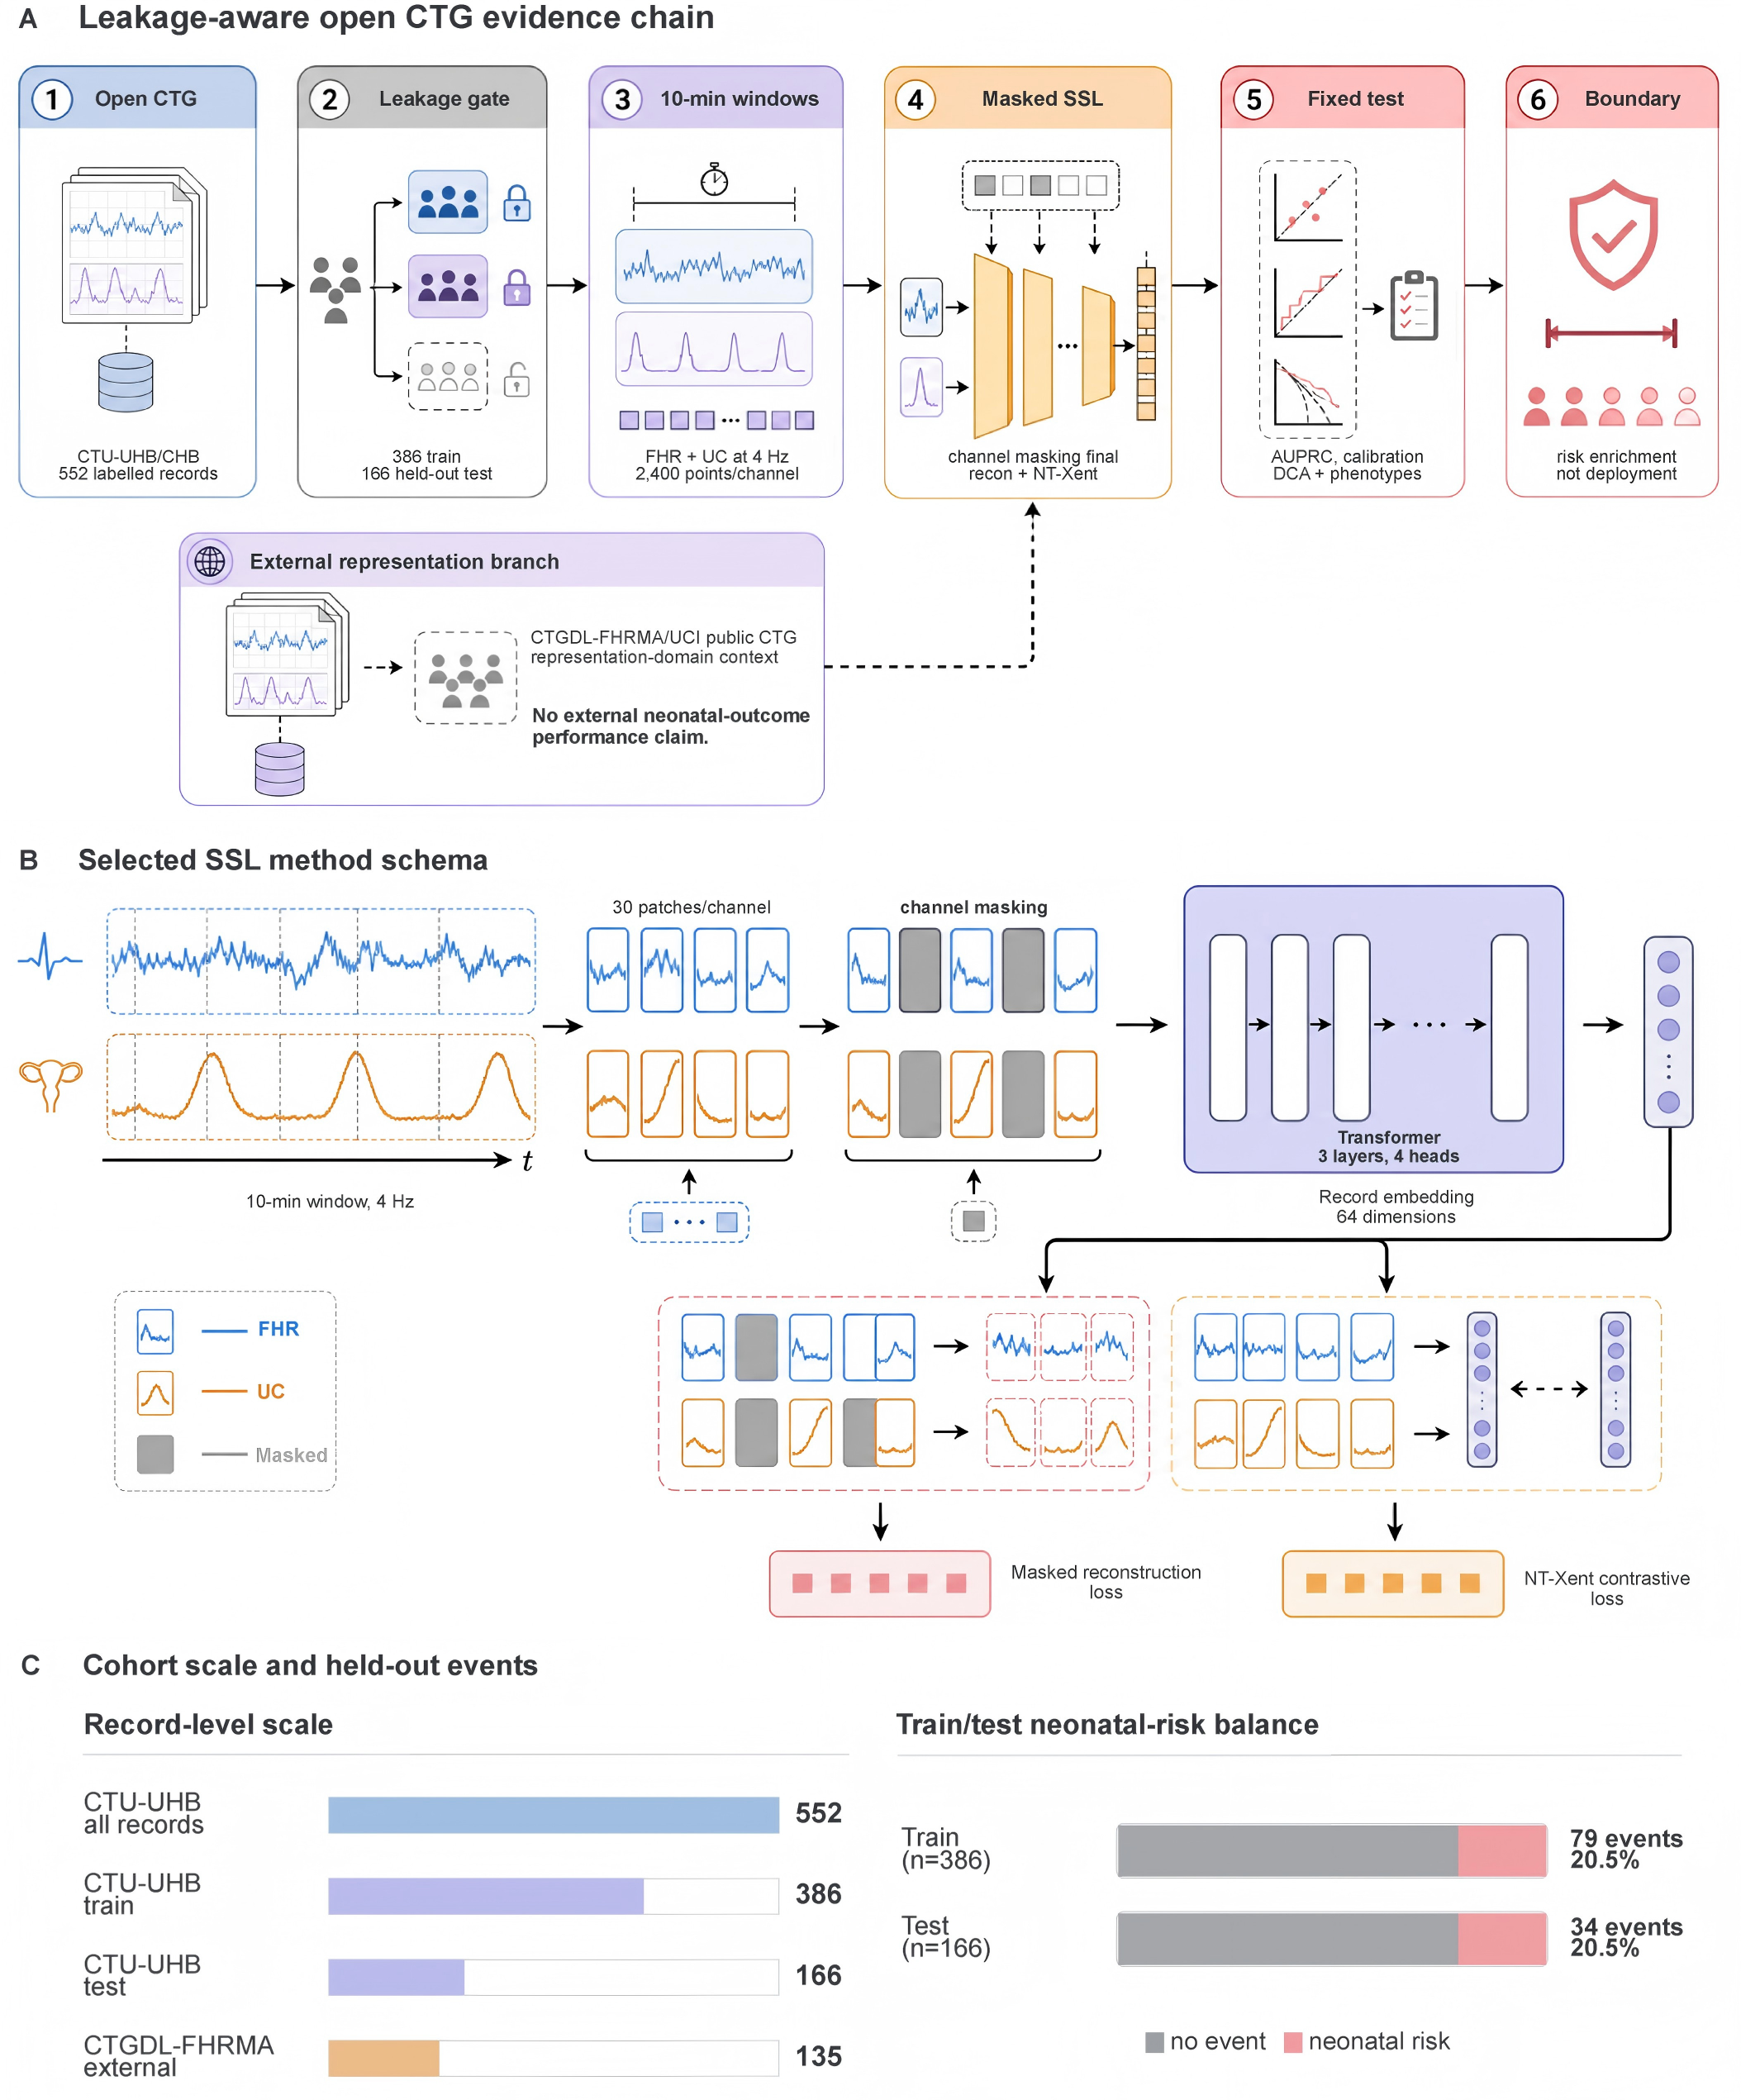
\includegraphics[width=\textwidth,height=0.78\textheight,keepaspectratio]{figures/Figure_1_study_design_pipeline.png}
              
              \caption{\textbf{Leakage-controlled open-data workflow for self-supervised CTG representation learning.} (A) Evidence chain from public CTU-UHB/CTU-CHB intrapartum CTG records through record-level train/test separation, 10-minute two-channel FHR/UC windows sampled at 4 Hz, channel-masking self-supervised pretraining, held-out risk enrichment, phenotype interpretation, recalibration and decision-curve analysis. The CTGDL-FHRMA/UCI branch is used only for representation projection and domain-shift context, because external neonatal-outcome labels were not analysed. (B) Selected SSL method: 30 non-overlapping patches per channel are channel-masked, encoded with a compact PatchTST-style transformer, and optimized with masked-reconstruction plus NT-Xent contrastive objectives to produce a 64-dimensional record embedding. (C) Cohort scale and event balance for the 552-record CTU-UHB cohort, the 386-record training split, the 166-record held-out split and the 135-record CTGDL-FHRMA external representation set.}\label{fig:study_design}
              \end{figure}


\clearpage
\begin{figure}[p]
              \centering
              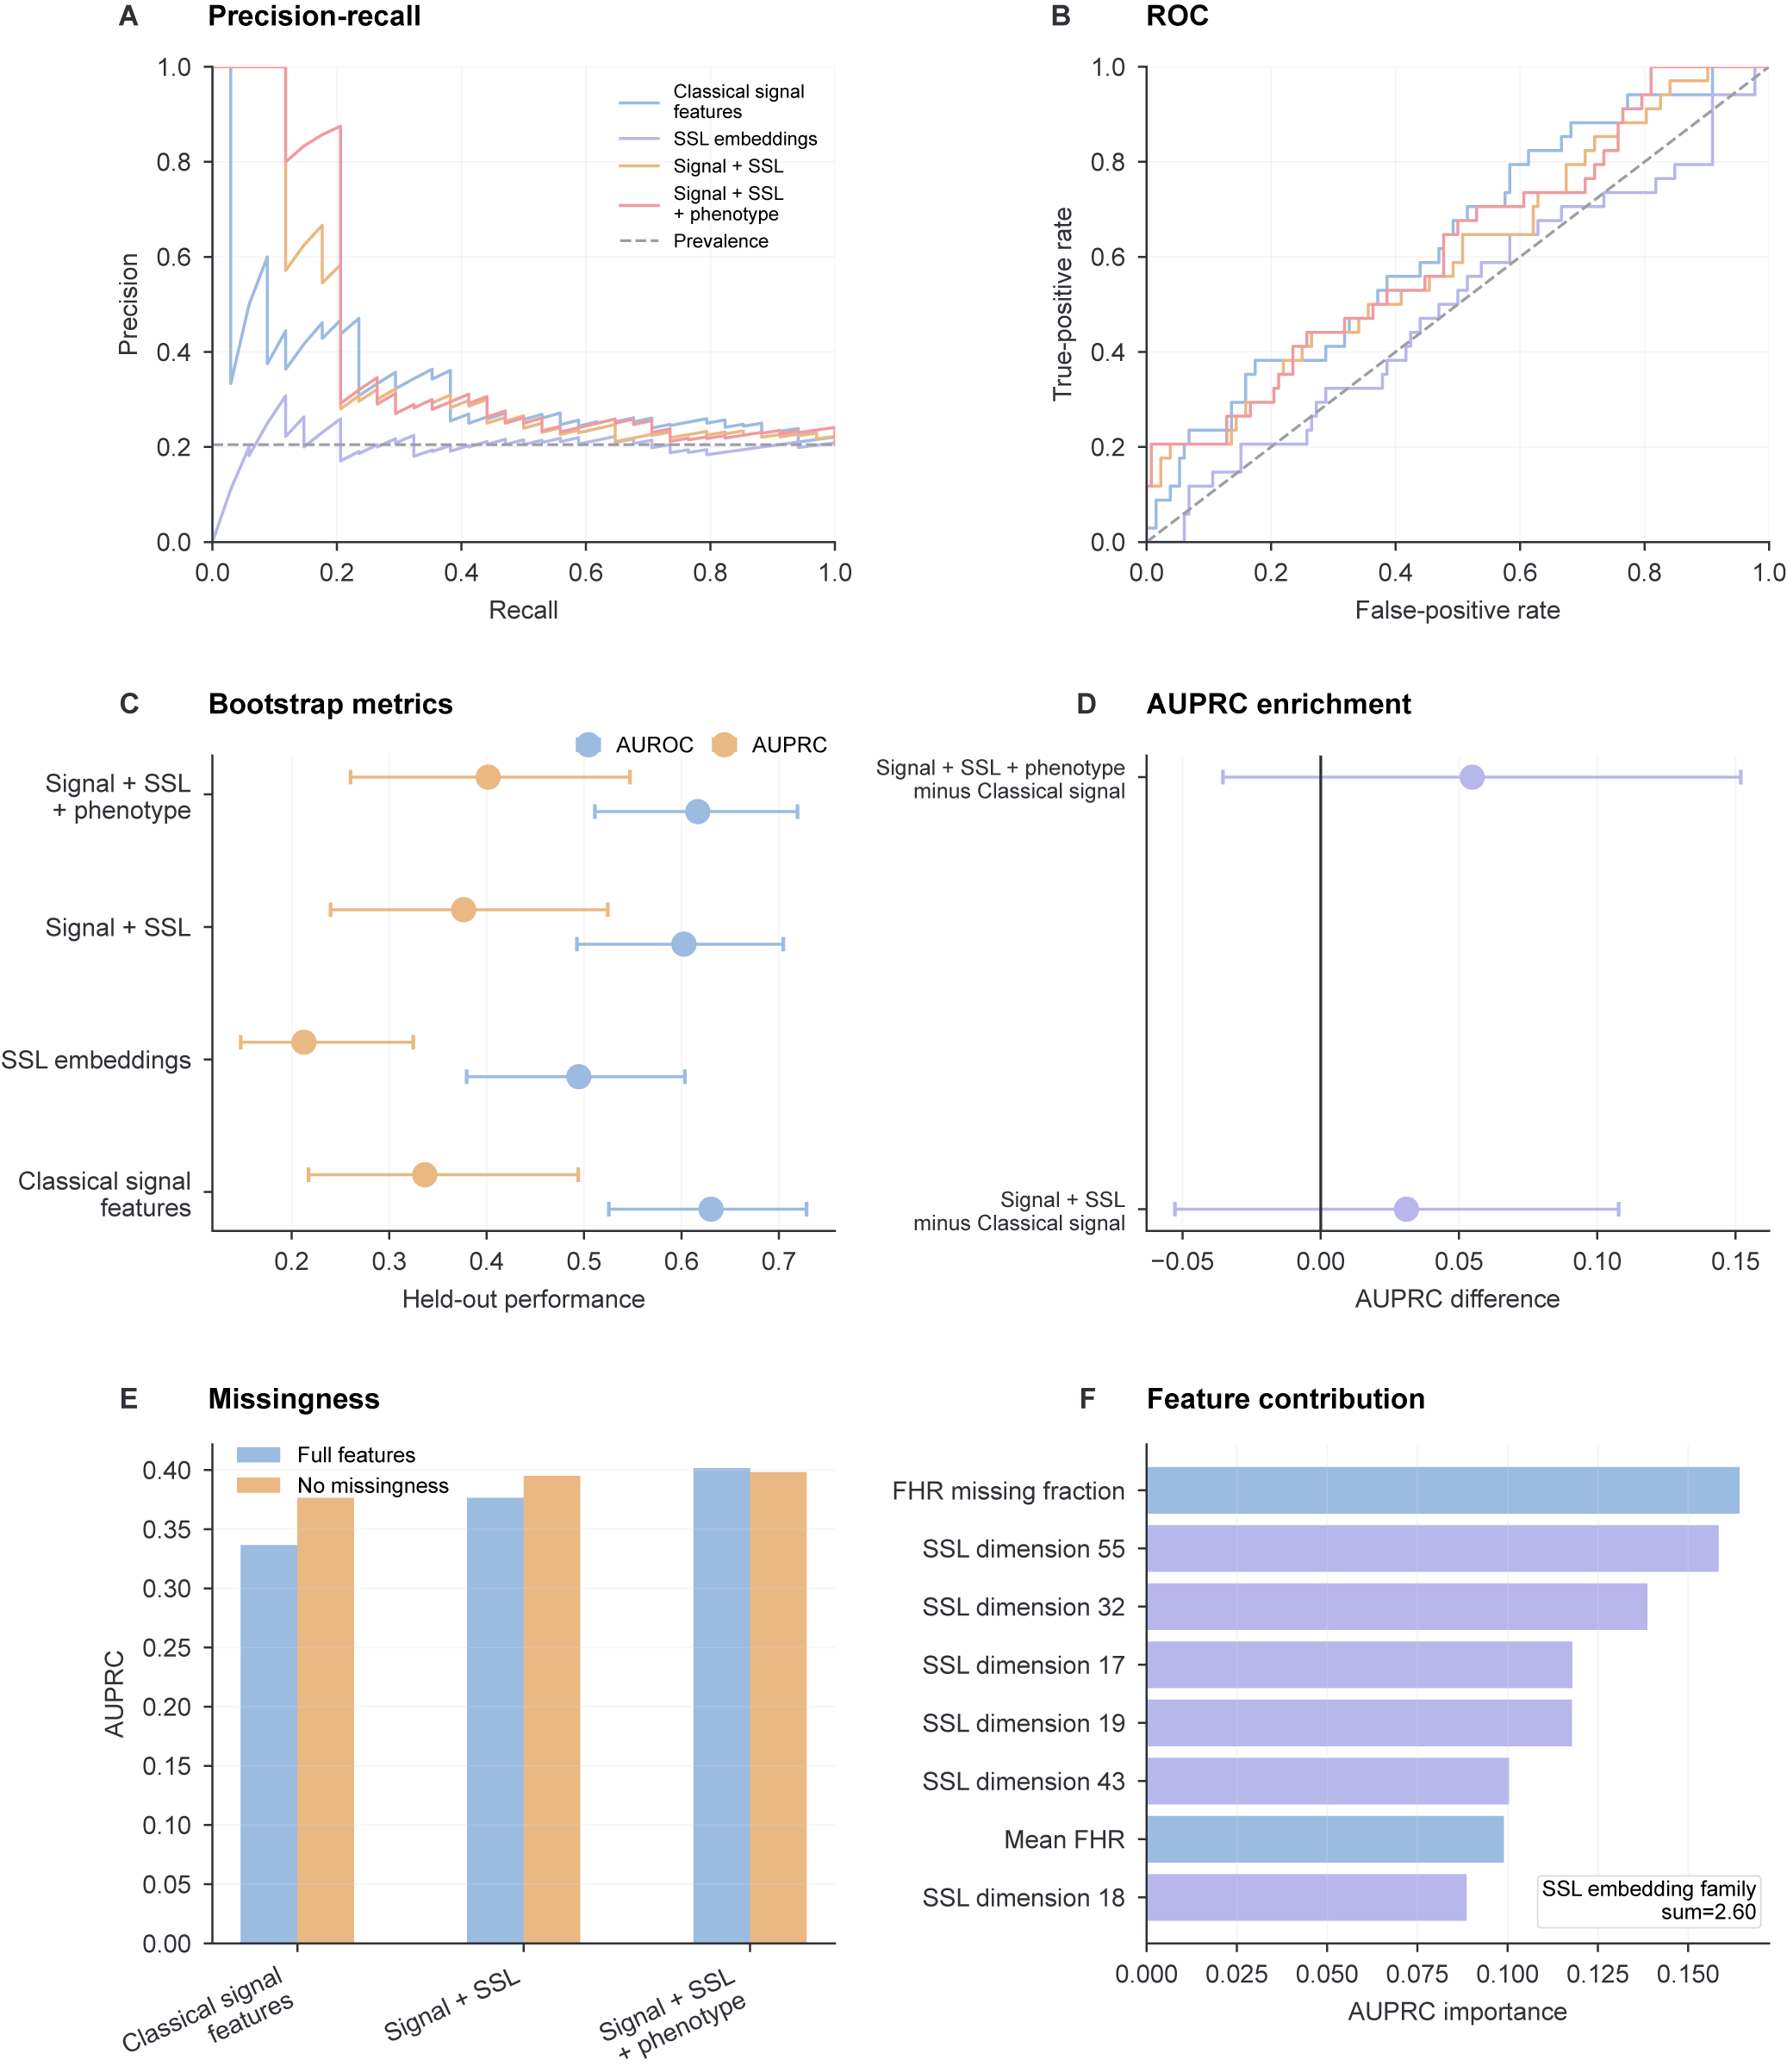
\includegraphics[width=\textwidth,height=0.81\textheight,keepaspectratio]{figures/Figure_2_model_validation_and_explanation.png}
              
              \caption{\textbf{Held-out model validation, uncertainty and feature contribution.} (A,B) Precision-recall and ROC curves in the 166-record CTU-UHB held-out set comparing classical signal features, SSL embeddings, signal-plus-SSL and the final signal-plus-SSL-plus-phenotype model; the dashed precision-recall reference marks held-out prevalence. (C) Bootstrap AUROC and AUPRC estimates with 95\% intervals for the four feature sets. (D) Bootstrap AUPRC differences relative to classical signal features. (E) Missingness sensitivity after removing missingness indicators and related features. (F) AUPRC-based permutation importance for the final model, separating FHR/signal features from SSL embedding dimensions. Intervals crossing zero support interpreting SSL as a representation and enrichment layer rather than a statistically resolved discrimination-gain claim.}\label{fig:model_validation}
              \end{figure}


\clearpage
\begin{figure}[p]
              \centering
              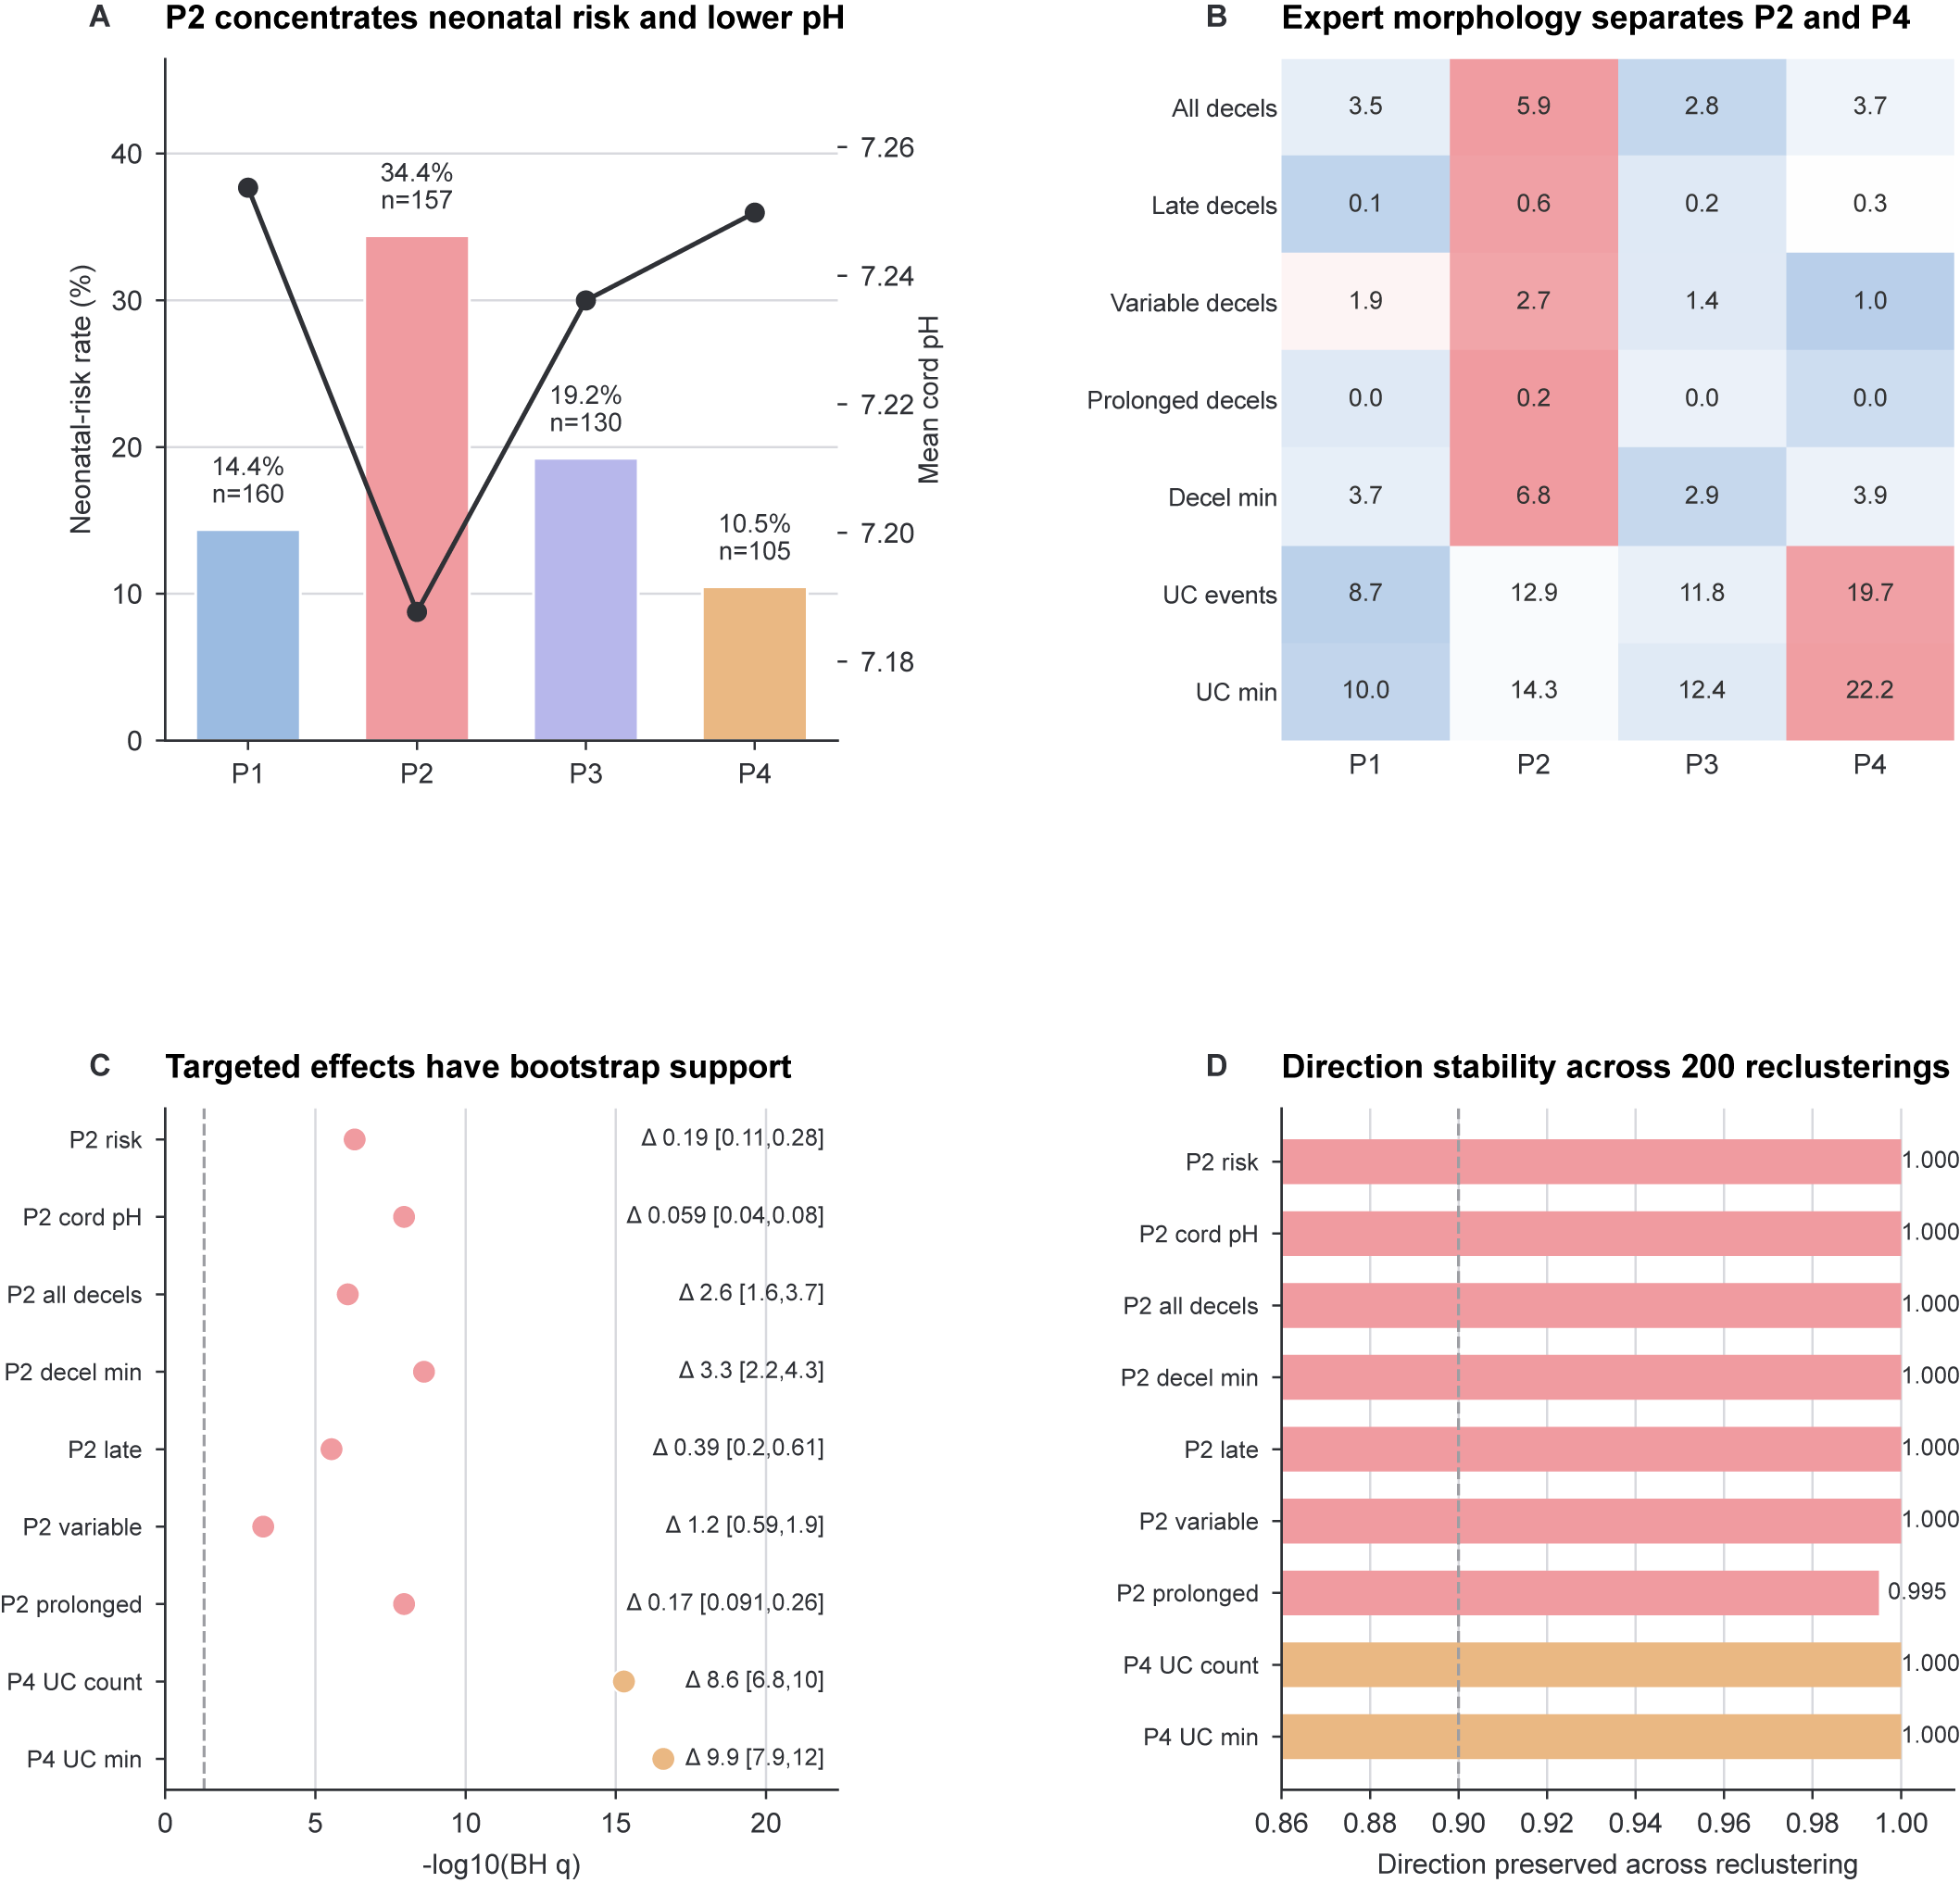
\includegraphics[width=\textwidth,height=0.82\textheight,keepaspectratio]{figures/Figure_3_dynamic_phenotype_prototypes.png}
              
              \caption{\textbf{Signal-derived dynamic phenotypes concentrate neonatal risk and interpretable CTG morphology.} (A) Neonatal-risk rate by phenotype with record counts, overlaid with mean cord pH, showing risk concentration and lower pH in phenotype P2. (B) Expert CTG morphology summaries across phenotypes, including all, late, variable and prolonged decelerations, minimum deceleration depth and uterine-contraction frequency/duration proxies. (C) Pre-specified P2 and P4 contrasts plotted as $-\log_{10}$ Benjamini-Hochberg-adjusted q values with bootstrap-supported effect estimates. (D) Direction stability for targeted phenotype effects across 200 perturbation reclusterings. These analyses are same-cohort descriptive phenotype evidence and do not establish causality or external outcome validation.}\label{fig:phenotypes}
              \end{figure}


\clearpage
\begin{figure}[p]
              \centering
              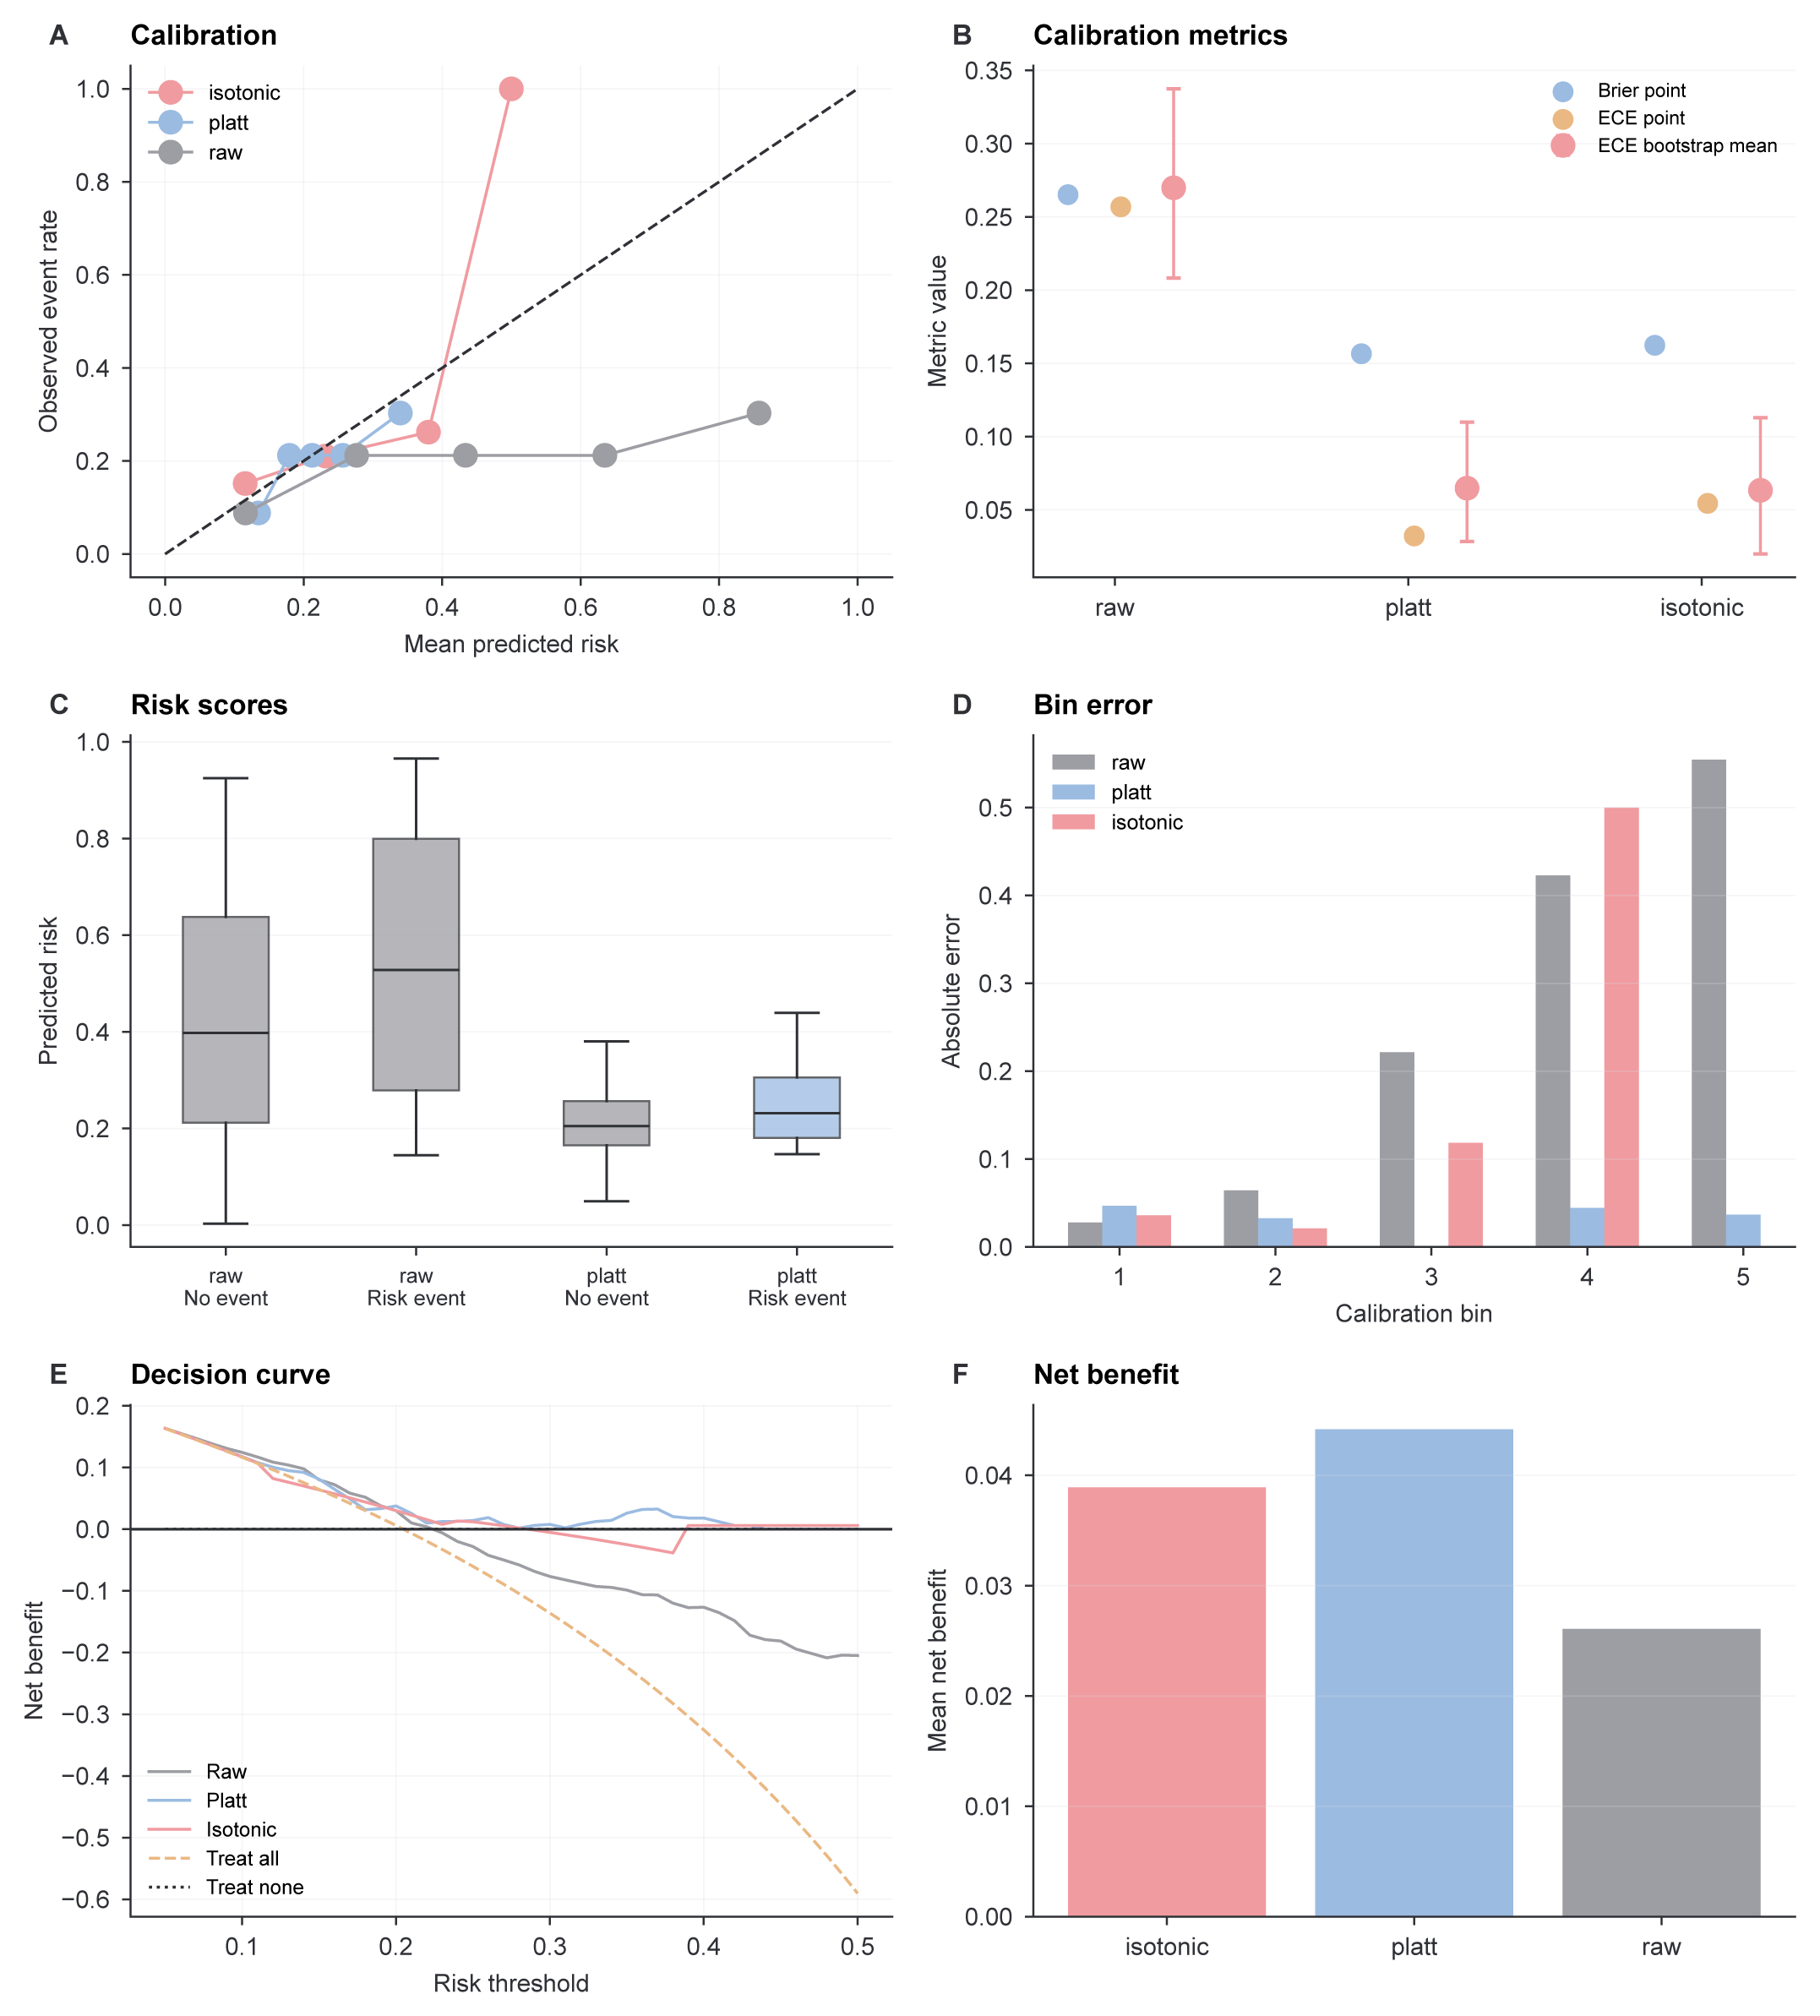
\includegraphics[width=\textwidth,height=0.81\textheight,keepaspectratio]{figures/Figure_4_recalibration_and_clinical_utility.png}
              
              \caption{\textbf{Cross-fitted recalibration and decision-curve analysis for absolute-risk interpretation.} (A) Calibration curves for raw, Platt-scaled and isotonic predictions in the held-out CTU-UHB set, compared with the ideal calibration diagonal. (B) Brier score, expected calibration error and bootstrap expected calibration error with 95\% intervals. (C) Predicted-risk distributions by event status before and after Platt recalibration. (D) Absolute bin-level calibration error for raw, Platt and isotonic predictions. (E) Decision curves across risk thresholds, with treat-all and treat-none references. (F) Mean net benefit across the 0.10--0.30 risk-threshold range. Platt recalibration improved absolute-risk calibration and threshold behaviour, whereas raw model scores should not be interpreted as calibrated neonatal-risk probabilities.}\label{fig:calibration_dca}
              \end{figure}

        \end{document}
